%\section{Graph Representation for RDF}
%
%\section{Deriving Incidence Graphs from Hypergraphs}
%
%A hypergraph $H$ may be represented by a bipartite graph $BG$ as follows: the sets $V$ and $E$ are the partitions of $BG$, and $(v_1, e_1)$ are connected with an edge if and only if vertex $v_1$ is contained in edge $e_1$ in $H$. Conversely, any bipartite graph with fixed parts and no unconnected nodes in the second part represents some hypergraph in the manner described above. This bipartite graph is also called incidence graph.
%
%The representation based on hypergraphs introduced in the previous section has the disadvantage that hypergraphs are not as common as conventional graphs. We now present a map that transforms hypergraphs representing RDF as studied above to a class of common graphs.
%
%As stated in the preliminaries chapter, hypergraphs can be represented by incidence matrices. Such a matrix can be understood as the node adjacency matrix of a bipartite graph. Thus, the idea is to represent RDF by means of bipartite graphs.
%
%Hypergraph incidence matrices represent membership of a node in an edge with a `1' in the corresponding entry (see Figure 6.2). In the case of the hypergraph representing an RDF Graph, the nodes of an edge are ordered. This ordering must be preserved in the incidence matrix: instead of using an integer according to the occurrence of a node in an edge, we choose to label them by S, P or O to represent the role (subject, predicate, or object) of the information resource in that statement-edge.
%
%Hence, when deriving the bipartite incidence graph of this incidence matrix, an edge will be added for every S, P, O entry of the matrix, and this edge will be labeled with the corresponding character. Thus, the only difference between the graph derived from the incidence matrix of any hypergraph and an RDF Graph hypergraph is the fact that each edge has one out of three labels.
%
%\begin{figure}[ht]
%\centering
%\begin{minipage}[c]{0.58\textwidth}\centering
%\[ \bordermatrix{ ~       &  \text{~a~}  &  \text{~b~}  &  \text{~c~}  &  \text{~d~}  &  \text{~e~}  &   \text{coa} &   \text{col} &   \text{inf} &   \text{fof} &   \text{subP}\cr
%                  E_1~~   &   1   &   1   &       &       &       &       &   1   &       &       &       \cr
%                  E_2~~   &       &   1   &   1   &       &       &   1   &       &       &       &       \cr
%                  E_3~~   &   1   &       &       &   1   &       &       &       &   1   &       &       \cr
%                  E_4~~   &       &       &       &   1   &   1   &       &       &       &   1   &       \cr
%                  E_5~~   &       &       &       &       &       &   1   &   1   &       &       &    1}
%\]
%\end{minipage}
%\hfill
%\begin{minipage}[c]{0.38\textwidth}\centering
%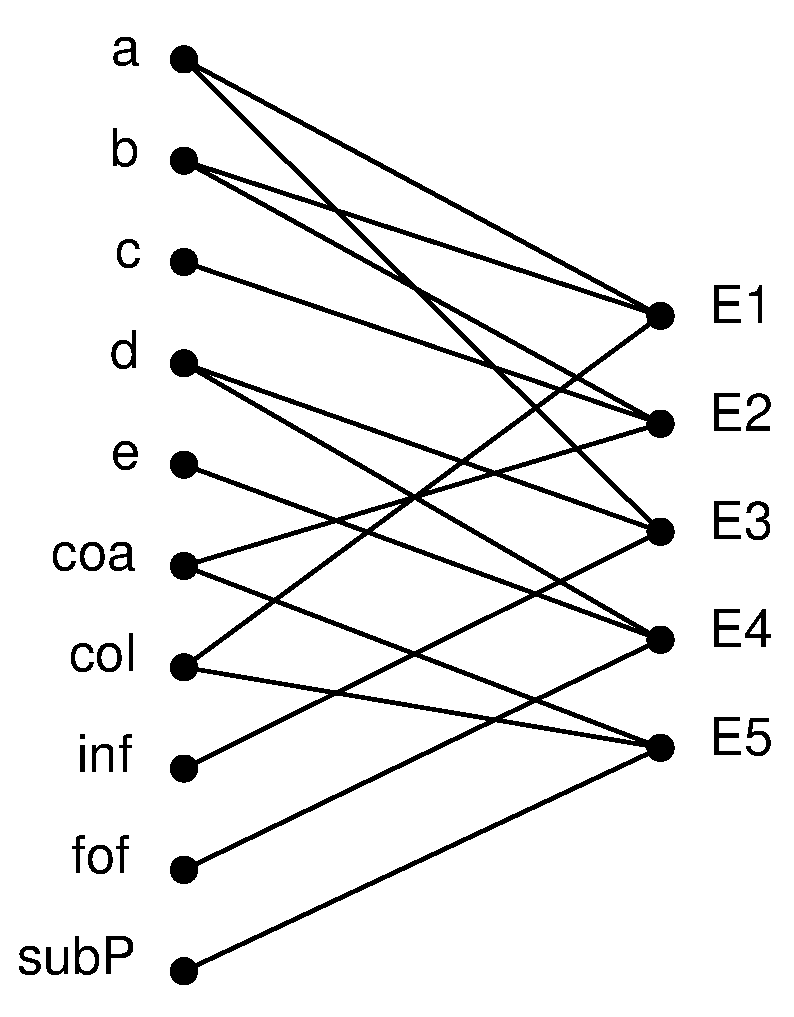
\includegraphics[width=.7\textwidth]{fig/BG-black.eps}
%\end{minipage}
%\caption{Incidence matrix representing the hypergraph of Example 6.1 and the corresponding incidence graph. In the case of an ordered hypergraph, matrix entries will indicate the position of the occurrence of the node in the edge. This section presented the underlying idea for representing RDF by bipartite graphs. In the following, the map will be formally introduced.}
%\end{figure}
%
%
%\section{Mapping RDF Graphs to Bipartite Graphs}
%
%Before formally defining the map from RDF Graphs to these incidence graphs, we study the graph class which is the range of this transformation.
%
%Definition 13 (Bipartite Labeled Graphs): Let $\mathcal{B}$ be the set of bipartite labeled graphs $G = (V \cup St,E, nl, el), V \cap St = \emptyset$;, where each edge in E connects a node in V with a node in St, and el : E ! EL and nl : V ! NL are labeling functions. The elements of $V$ are called \emph{value nodes} and those of $St$ are \emph{statement nodes}. To allow multiple edges between nodes we understand $E$ as a set of edge elements and introduce functions stat : $E \rightarrow St$ and val : $E \rightarrow V$ which yield the statement node stat($e$) and the value node val($e$) which are connected by an edge $e$.
%
%The above defined set of graphs B represent the bipartite incidence graphs derivable from hypergraphs��although the naming of the node classes already reflects the intended usage. To specify the graphs to be obtained from hypergraphs
%representing RDF Graphs��that is, the incidence graphs of (a certain subset of) simple ordered 3-uniform hypergraphs��the following restrictions are made:
%
%Definition 14 (RDF Bipartite Graphs (RBG)): We define the graph class $\text{RBG} \subset \mathcal{B}$ as follows. Let $B = (V \cup St, E, nl, el) \in \text{RBG}$. The set of edge labels is $\text{EL} = {S, P,O}$ and the set of node labels NL is partitionable into the three sets uris($B$), blanks($B$), and lits($B$). Then it holds
%(1) for all $st \in St$ :
%\[degree(st) = \]
%and (2): for all $e \in E$ with $\emph{val}(e) = v$:
%\section{Direct Label Graph}
%In Section~\ref{sec:rdfgraph}, we describe the directed labeled graph representation for RDF and its shortcomings in illustrating schematic assertions on properties. We also describe the hypergraph representation for RDF that is able to overcome the problem. In this section,
%RDF triples can be visualized as a \emph{directed labeled graph},
%\begin{center}
%\ovalbox{subject} $\stackbin[]{predicate}{\xrightarrow{\hspace*{2cm}}}$ \ovalbox{object}\;,\\
%\end{center}
%where subjects and objects are represented as nodes, and predicates as edges. This graph model is straightforward and convenient in most of cases. But inconsistency arises when using triples to make assertions on predicates. The following example illustrates this point of view.
%
%
%
%Both solutions have problems. Allowing arcs connecting nodes with other arcs can lead to puzzling drawings. What is more, the graph drawn this way has sets of arcs and nodes which intersect, which does not correspond to the commonly accepted definition of graphs. Defining a graph representation which is not a graph reduces this task to visualization for humans and gives away advantages of a true graph representation.
%
%On the other hand, duplicating the visual representation of an information resource for its role as predicate (representation as edge label) and as subject / object (representation as node) has a disadvantage. Information about a property (its sub- and super-properties, its domain and range) are disconnected from the actual usage of the property. This might result in users drawing misleading conclusions; allowing such multiple occurrences of resources jeopardizes one of the most important aspects of graph visualization, which is the implicit assumption that the complete information regarding an entity in a graph is obtained by examining its place in the drawing and its incident edges. Furthermore, chapter 9 introduces the notion of connectivity, which is central to querying RDF data. Duplicating properties in the graph representation of an RDF Graph makes it unsuitable for the study of connectivity.
%
%However, it is not so much the ambiguity of the definition as the limitation of directed labeled graphs as such which causes problems in modeling RDF. RDF triples establish ternary relations which cannot be truly represented by the binary edges of classic graphs. Labeling the edges neglects the fact that properties are information resources in their own right, leading to the problem of either non-standard graphs or repeated occurrences of the same resource throughout the graph.
%
%Thus, it can be said that the graph-like nature of RDF is intuitively appealing, but its naive formalization as directed labeled graph presents problems inherent in this type of graph. The recognition of the insufficiency of binary edges to model RDF statements led to an approach based on ternary edges (hypergraphs),

%\section{Representing Domain Knowledge and Data using Graphs}
The interface between domain knowledge and data is achieved by employing the RDF model and by the fact that RDF allows a combined specification of both schema and data structured under this schema.

RDF's abstract triple syntax has a graph nature. Graphs are mathematical objects that enjoy wide-spread usage for many tasks, which include the visualization and analysis of data for humans, mathematical reasoning, and the implementation as a data structure for developing data mining algorithms. Besides the common graph-theoretic model of RDF as labeled, directed multi-graphs, Hayes has established that RDF can be also represented as hypergraphs (bipartite graphs)~\cite{GraphModelRDF}. This result constitutes an important aspect of the theoretical basis of this proposal and is discussed in sections below. We propose to use the graph-based representation for RDF as a combined information source of both domain knowledge and data for different mining tasks, including association rule mining, classification, clustering and so forth.

\section{Graph Representation for Domain Knowledge}
Graph-based approaches for representing knowledge have long been used in philosophy, psychology, and linguistics. The computer counterpart to this means is the so-called \emph{semantic network} that represents knowledge in patterns of interconnected nodes and arcs which were first developed for artificial intelligence and machine translation.

The semantic network, and graph-based approaches for KR in general, are motivated by the desirable qualities of graph for both modeling and computation. From a modeling viewpoint, basic graphs are easily understandable by users, and it is always possible to split up a large graph into smaller ones while keeping its semantics. From the computational viewpoint, graph is one of the most studied objects in mathematics. Considering graphs instead of logical formulas provides another view of knowledge constructs (\eg, some notions like path, cycle, or connected components are natural on graphs) and provides insights to algorithmic ideas~\cite{CheinMugnier08}. In light of these motivations, what is common to all semantic networks is a declarative graphic representation that can be used either to represent knowledge or to support automated systems for reasoning about knowledge.

Among all variants of semantic networks, we emphasize the most on the usage of definitional networks to incorporate domain knowledge in data mining. The kind of knowledge that are best captured by this kind of network is subsumption hierarchy, on which a distance (similarity) measure can be reasonably defined. Such measure is essential in many data mining tasks. It is possible to extend, in a straightforward manner, data mining algorithms that depend on analyzing distances between entities in factual knowledge to work with distances between those in ontological knowledge.

In addition, one of the most prominent KR formalism families among current systems of definitional networks, description logics (DLs), formerly called terminological logics or concept languages, have been a successful attempt to combine well-defined logical semantics with efficient reasoning~\cite{Sowa91principlesof}. They are derived from an approach proposed by Woods~\cite{woods75link} and implemented by Brachman~\cite{Brachman91livingwith} in a system called Knowledge Language One (KL-ONE). Recent description logics are DAML+OIL~\cite{Horrocks02daml+oil} and its successor OWL, which are intended for representing knowledge in the semantic web~\cite{Berners-Lee01}--a giant semantic network that spans the entire Internet.

OWL ontologies can be used along with information written in RDF, and OWL ontologies themselves are primarily exchanged as RDF documents. RDF's abstract triple syntax has a graph nature. The RDF graph is defined as follows according to the W3C specification for RDF semantics~\cite{Hayes_rdf2004}:

\begin{mydef}[\textbf{RDF Graph}]
An RDF graph is defined as a set of RDF triples. A subgraph of an RDF graph is a subset of the triples in the graph. A triple is identified with the singleton set containing it, so that each triple in a graph is considered to be a subgraph. A proper subgraph is a proper subset of the triples in the graph. A ground RDF graph is one with no blank nodes.
\end{mydef}

RDF triples can be visualized as a \emph{directed labeled graph} as follows:
\begin{center}\ovalbox{subject} $\stackbin[]{predicate}{\xrightarrow{\hspace*{2cm}}}$ \ovalbox{object}\;,\end{center}
where subjects and objects are represented as nodes, and predicates as edges. The directed labeled graph model for RDF is straightforward and convenient in most cases. But inconsistency arises when using triples to make assertions on predicates. The directed labeled graph model of RDF makes the artificial distinction between resources and properties, which may cause inconsistency in the graph representation. The following example illustrates this point of view.

\begin{figure}[tbh]
\begin{center}
\begin{tabular}{ccc}
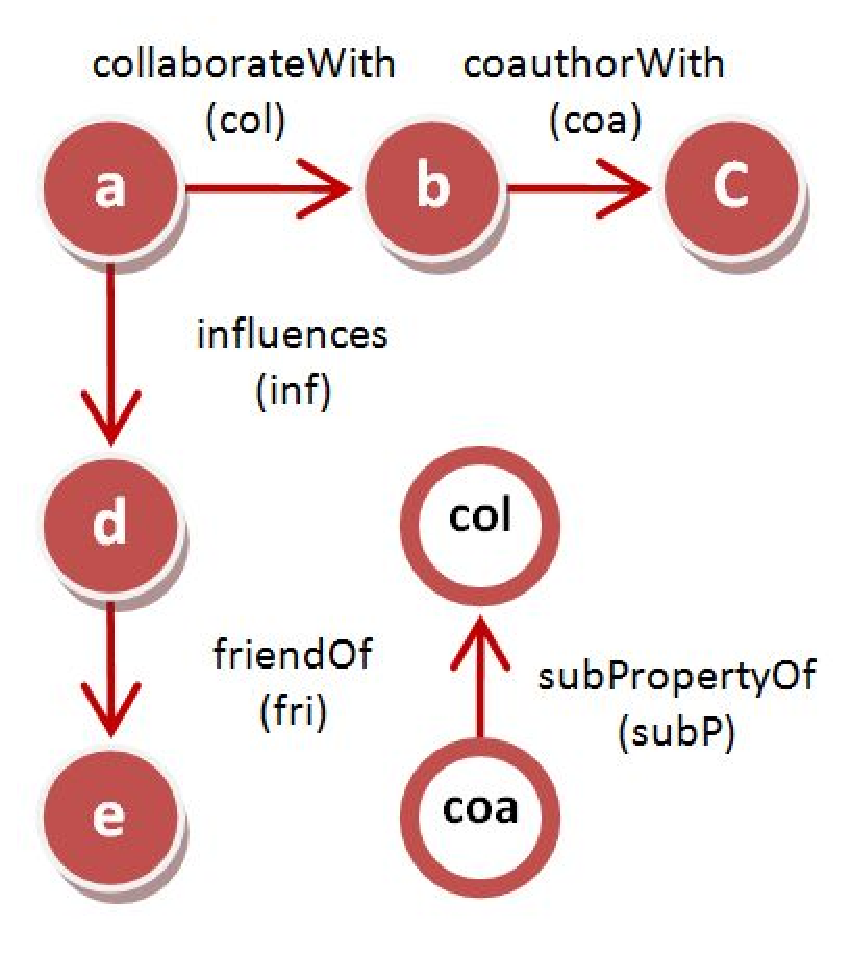
\includegraphics[width=.25\textwidth]{fig/reg_graph.eps} & &
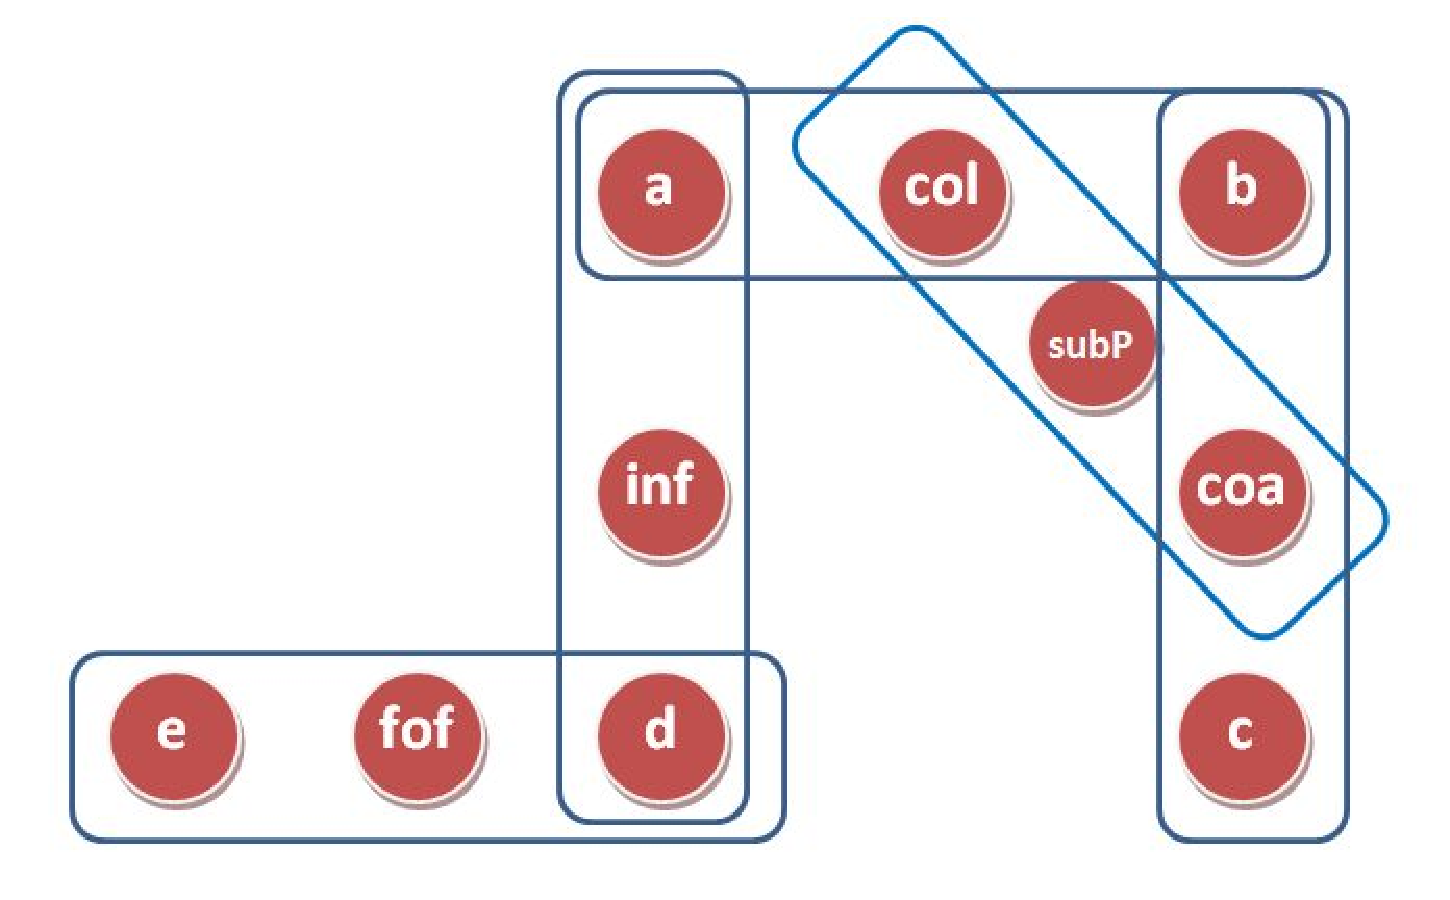
\includegraphics[width=.43\textwidth]{fig/hypergraph.eps}\\
(A) & & (B)\\
\end{tabular}
\end{center}
\caption{\label{fig:graphcomp} An example of nodes connected by different links and some relationship between the links, represented by A) a simple graph, and B) a hypergraph.}
\end{figure}

\begin{myexp}[\textbf{Inconsistent representation of RDF directed labeled model}]
\label{graphcomp}
In this example, a set of RDF statements is asserted to describe the relationship among a group of people. The information expressed include two different levels, i.e., the meta (ontological) data and factual data. The factual data level consists of following statements: $\langle a~ collaborate~ b\rangle$, $\langle b~ coauthor~ c\rangle$, $\langle a~ influence~ d\rangle$ and $\langle d~ friendOf~ e\rangle$. The meta-data level contains one single statement asserting that $coauthor$ is a sub-property of $collaboration$: $\langle coauthor~ subProperty~ collaboration\rangle$. In this case, the representation of $collaboration$ and $coauthor$ is inconsistent. They are represented as nodes at the factual data level and edges at the meta-data level (see Figure~\ref{fig:graphcomp}(A)).
\end{myexp}

To overcome this, Hayes et al.~\cite{GraphModelRDF} proposed to model RDF as a \emph{hypergraph}. A hypergraph~\cite{Hypergraph} is a generalization of a traditional graph where edges, called hyperedges, can connect more than two vertices. If each edge in a hypergraph covers the same number of nodes, it's called $r$-uniform hypergraph, $r$ being the number of nodes on each edge. Any RDF Graph can be represented by a simple ordered 3-uniform hypergraph, in which an RDF triple corresponds to a hypergraph edge, the nodes being the subject, predicate and object in this order. In this way, both meta-data and data level statements can be integrated in a consistent model.

In Fig.~\ref{fig:graphcomp}(B), the information in the Example~\ref{graphcomp} is represented by a hypergraph and the inconsistency in the directed labeled graph representation is eliminated.

\begin{mydef}[\textbf{Hypergraph}]
Formally, a hypergraph $G = (V,E)$, is a pair in which $V$ is the vertex set and $E$ is the hyperedge set where each $e \in E$ is a subset of $V$. A weighted hypergraph is a hypergraph that has a positive number $w(e)$ associated with each hyperedge $e$; called the weight of hyperedge $e$: Denote a weighted hypergraph by $G = (V,E,w)$. The degree of a vertex $v \in V$, $d(v)$, is defined as $d(v) = \sum_{v\in V, e\in E}{w(e)}$. The degree of a hyperedge $e$, denoted as $\delta(e)$, is the number of vertices in $e$, i.e. $\delta(e)=|e|$. A hyperedge $e$ is said to be incident with a vertex $v$ when $v \in e$. The hypergraph incidence matrix $\mathbf{H} \in \mathbb{R}^{|V| \times |E|}$ is defined as
\begin{equation}
\notag h(v,e)=\left\{\begin{array}{cl}
	   1, & v \in e \\
	   0, & otherwise
	   \end{array}\right.
\end{equation}
Throughout the rest of the paper, the diagonal matrix forms for $\delta(e)$, $w(e)$, $d(v)$ are denoted as $\mathbf{D}_e$, $\mathbf{W} \in \mathbb{R}^{|E|}$, and $\mathbf{D}_v \in \mathbb{Z}^{|V|}$, respectively.
\end{mydef}

A hypergraph $G = (V, E)$ can be transformed to a \emph{bipartite graph} $BG$ as follows:

\begin{mydef}[\textbf{Transformation from RDF hypergraph to RDF bipartite graph}]
Let the sets $V$ and $E$ are the partitions of $BG$. The node pair $(v_1, e_1)$ is connected with an edge if and only if vertex $v_1$ is contained in edge $e_1$ in $H$. Conversely, any bipartite graph with fixed parts and no unconnected nodes in the second part represents some hypergraph in the manner described above. This bipartite graph can be represented by incidence matrices. Such a matrix can be understood as the node adjacency matrix of a bipartite graph.
\end{mydef}
\begin{figure}[tbh]
\centering
\begin{minipage}[c]{0.58\textwidth}\centering
\[ \bordermatrix{ ~       &  \text{~a~}  &  \text{~b~}  &  \text{~c~}  &  \text{~d~}  &  \text{~e~}  &   \text{coa} &   \text{col} &   \text{inf} &   \text{fof} &   \text{subP}\cr
                  E_1~~   &   1   &   1   &       &       &       &       &   1   &       &       &       \cr
                  E_2~~   &       &   1   &   1   &       &       &   1   &       &       &       &       \cr
                  E_3~~   &   1   &       &       &   1   &       &       &       &   1   &       &       \cr
                  E_4~~   &       &       &       &   1   &   1   &       &       &       &   1   &       \cr
                  E_5~~   &       &       &       &       &       &   1   &   1   &       &       &    1}
\]
\end{minipage}
\hfill
\begin{minipage}[c]{0.38\textwidth}\centering
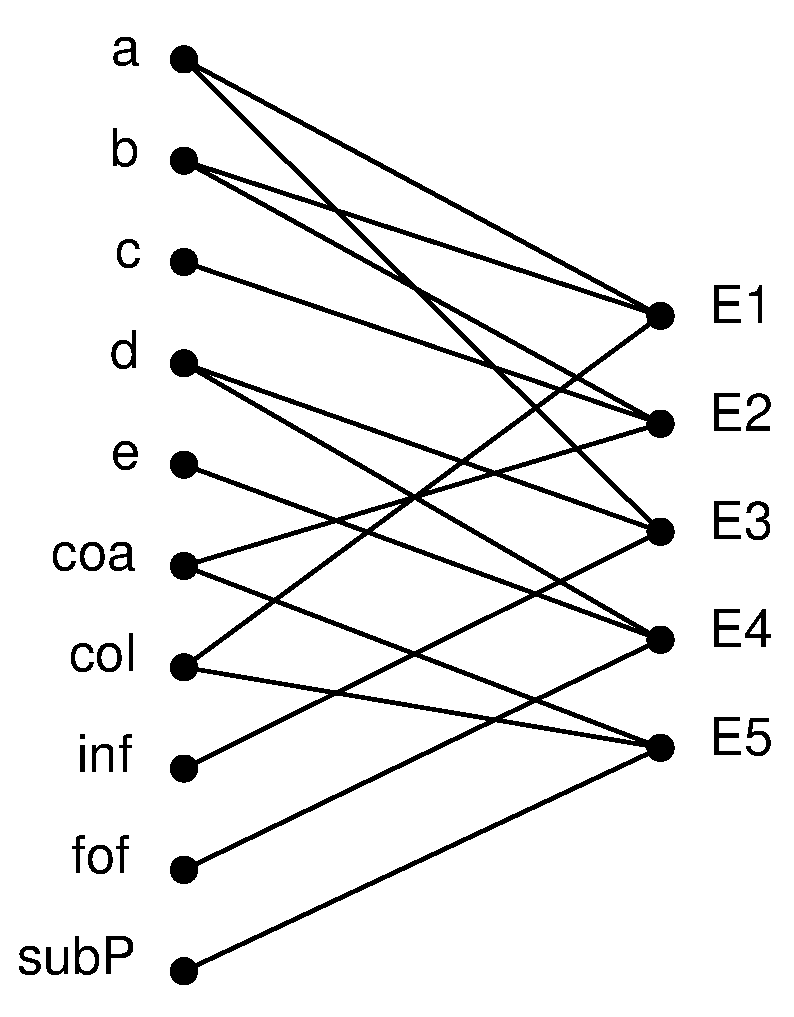
\includegraphics[width=.7\textwidth]{fig/BG-black.eps}
\end{minipage}
\caption{\label{fig:incidence}Incidence matrix representing the hypergraph of figure~\ref{fig:graphcomp}(B) and the corresponding incidence graph.}
\end{figure}

RDF bipartite graphs have many desirable properties for developing intuitive mining algorithms. Thus, the we propose to use bipartite graphs to represent domain knowledge and data expressed in RDF.

\begin{myexp}[\textbf{Hypergraph incidence matrix and corresponding bipartite graph}]
\label{incidence}
Figure~\ref{fig:incidence} (A) shows the incidence matrix according to the hypergraph in Figure~\ref{fig:graphcomp} for Example~\ref{graphcomp}. Figure~\ref{fig:incidence} (B) shows the corresponding bipartite graph. Hypergraph incidence matrices represent membership of a node in an edge with a ``1" in the corresponding entry.
\end{myexp}

Example~\ref{incidence} illustrates the general method that can be applied to all hypergraphs to transform to their bipartite graph form. In the case of a hypergraph representing an RDF Graph, since nodes in a RDF statement are ordered (subject followed by predicate then object), this ordering must be preserved in the incidence matrix. A \emph{labeled bipartite graph} can be derived to further capture the ordering and roles of nodes.

\begin{mydef}[\textbf{RDF labeled bipartite graph}]
In the hypergraph incidence matrix, instead of using ``1/0'' according to the occurrence of a node in an hyperedge, we choose to label them by S, P or O to represent the role (subject, predicate, or object) of the node in that underlying RDF statement--edge. Hence, when deriving the bipartite graph of a hypergraph incidence matrix, an edge will be added for every S, P, O entry of the matrix, and this edge will be labeled with the corresponding character (S, P, or O). Thus, the only difference between the graph derived from the incidence matrix of any hypergraph and an RDF Graph hypergraph is the fact that each edge has one out of three labels~\cite{GraphModelRDF}.
\end{mydef}

In the rest of the proposal, when we use RDF bipartite graph, we mean RDF labeled bipartite graph for short.

\begin{myexp}[\textbf{RDF labeled bipartite graph}]
Figure~\ref{fig:graphcomp-bio} illustrates an example of RDF hypergraph represented as labeled bipartite graph. The left side shows a portion of an ontology in biomedical domain on zebrafish anatomy~\cite{ZFA} visualized as a directed labeled graph. Two different relationships are depicted in the figure, namely, ``subClassOf" and ``part\_of". The corresponding labeled bipartite graph representation is shown on the right side. Circle nodes are the \emph{statement nodes} representing the RDF statements. Each statement node is connected to three \emph{value nodes} representing the three components of a statement (subject, predicate, and object). Edge labels S, P, and O indicate the role of the value nodes in the statement.
\end{myexp}

\begin{figure}[tbh]
\centering
\begin{minipage}[c]{0.35\textwidth}\flushright
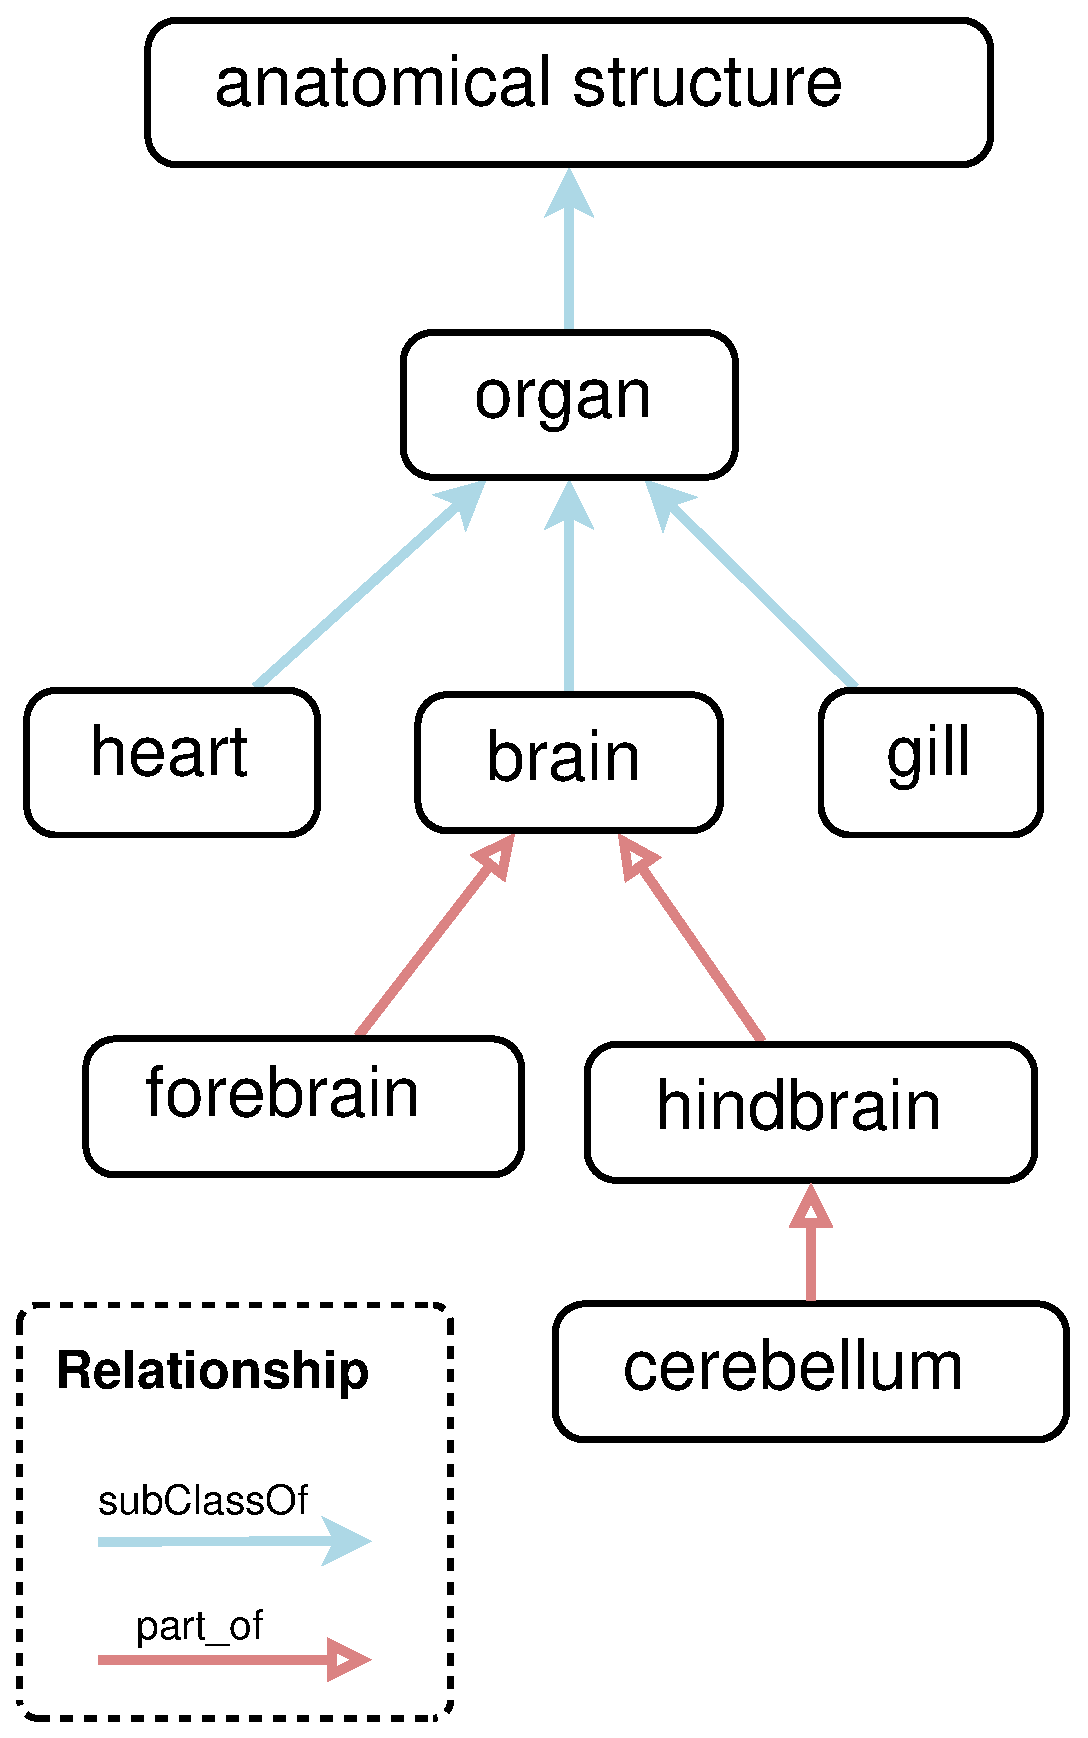
\includegraphics[width=.7\textwidth]{fig/DLG-bio.eps}
\end{minipage}\hfill
\begin{minipage}[c]{0.6\textwidth}\centering
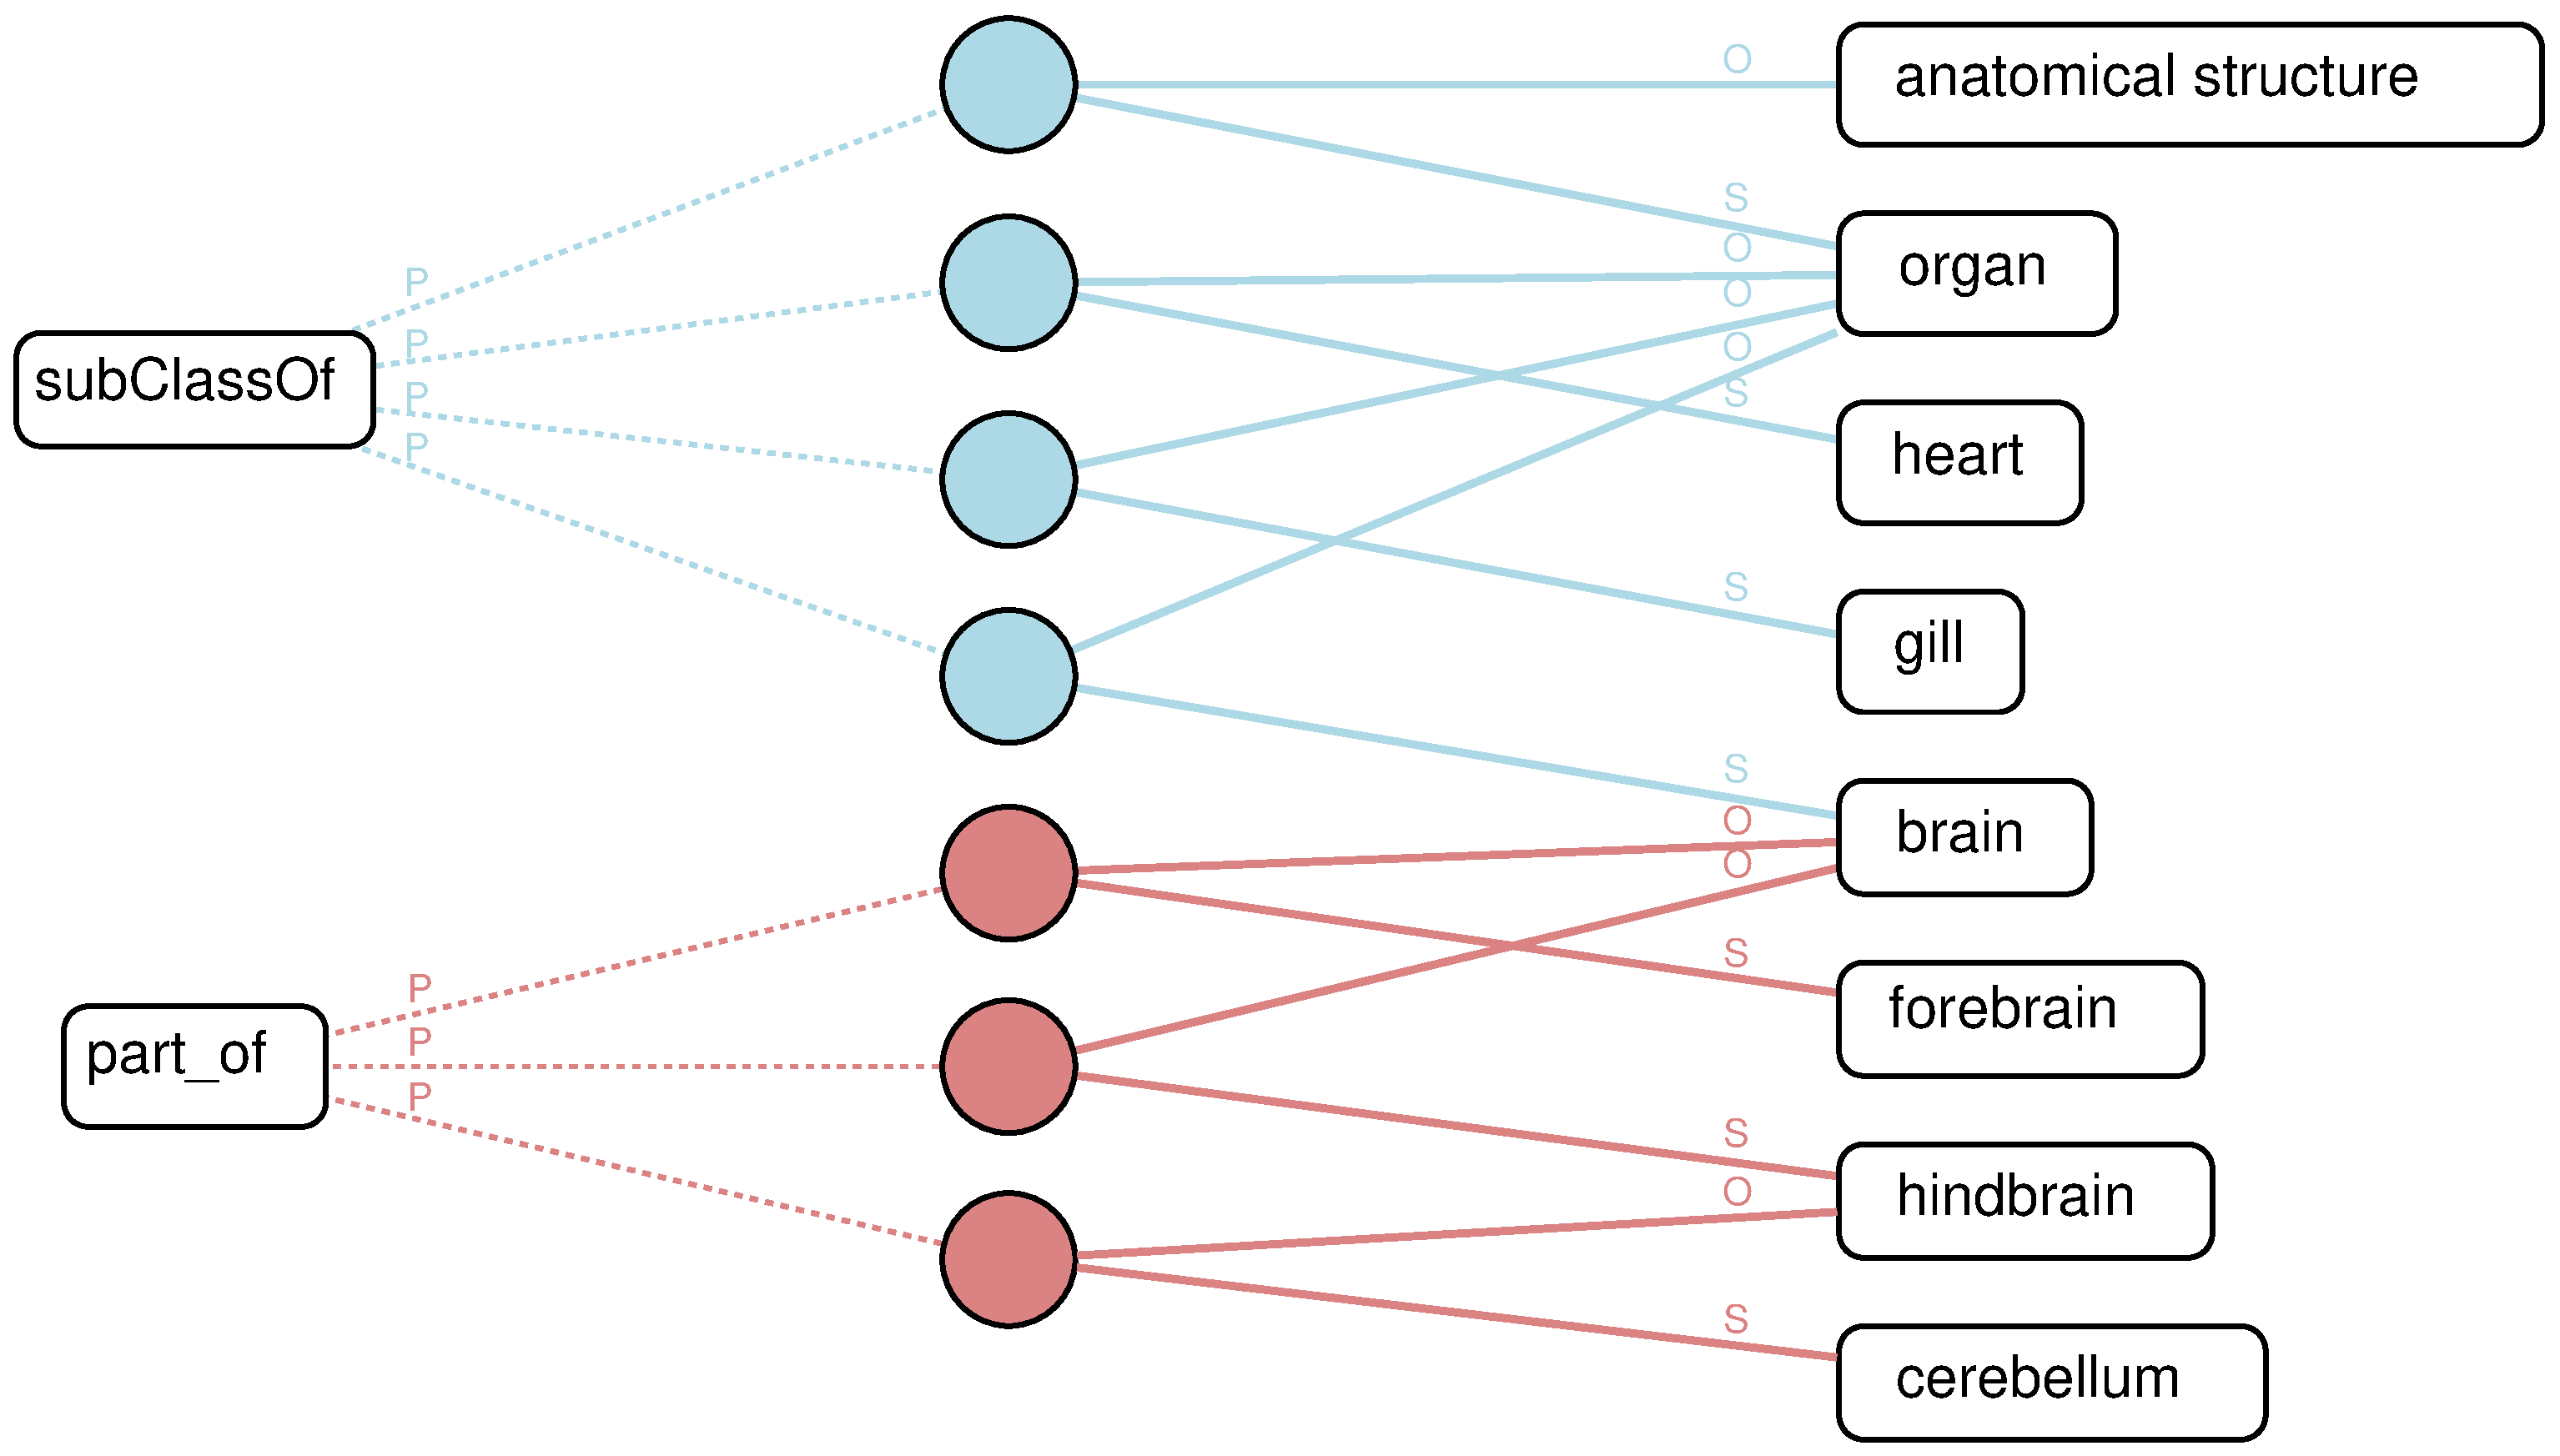
\includegraphics[width=\textwidth]{fig/BG-bio.eps}\\
\end{minipage}
\caption{\label{fig:graphcomp-bio} A portion of a zebrafish anatomy ontology represented as a directed labeled graph (A) and a RDF bipartite graph (B)}
\end{figure}

\section{Graph Representation for Relational Structure}
\label{sec:graph-rep-for-rdb}
Various graph representation for relational structure has been proposed in literature to tackle different data mining tasks. In the case of frequent itemset mining, a set of objects with the co-occurrence relationship can be represented as directed or undirected graphs (see the example in Figure~\ref{fig:hg_and_rg}).

Another way to represent relational structure is to first transform it to RDF, and by utilizing the graph nature of RDF, the relational structure can then be represented as graphs. Mapping from RDB to RDF has gained increasing attention and led to implementation of generic mapping tools as well as domain--specific applications.  The W3C launched the RDB2RDF incubator group to explore issues involved in mapping RDB to RDF. A work-in-progress survey paper has been published documenting approaches in this field~\cite{RDB2RDF}.

%We can classify the methods used to generate the mappings between RDB and RDF into two categories:
A straightforward method for mapping RDB to RDF is discussed by Berners Lee~\cite{TBL98} as defined in the following.

\begin{mydef}[\textbf{Context--independent mapping from RDB to RDF}]
Without linking to any explicit definition of domain semantics (such as those defined in domain ontologies), a RDB can be transformed to RDF following the steps below:
\begin{enumerate}
\label{auto-map}
\item A RDB row is a RDF subject node.
\item The column name of a RDB table is a predicate node.
\item A RDB table cell is an object node.
\end{enumerate}
\end{mydef}

Many systems leverage these mappings to automatically generate mappings between RDB and RDF. Even though these automatically generated mappings often do not capture complex domain semantics that are required by many applications, these mappings can serve as a useful starting point to create more customized, domain--specific mappings.

\begin{myexp}[\textbf{RDF bipartite graph for a nominal-valued RDB}]
Table~\ref{tbl:nominal-rel} (A) shows a relational table with nominal features (columns). The table has $m$ rows, each one annotated on the border with labels $r_1 \ldots r_m$, and $n$ columns named $f_1 \ldots f_n$. Applying the steps in Definition~\ref{auto-map} for mapping RDB to RDF mapping, the corresponding RDF statements are listed in Table~\ref{tbl:nominal-rel} (B). From these statements, a RDF bipartite graph is derived, shown in Figure~\ref{fig:BG-relational-nominal}, as the graph representation for the underlying relational table in Table~\ref{tbl:nominal-rel} (A).
\end{myexp}

\begin{table}[ht]
\begin{minipage}[c]{0.4\linewidth}\begin{flushright}
\begin{tabular}{ c | c | c | c |}
\cline{2-4}
	~   & $f_1$	    & $\cdots$  & $f_n$   \\
\cline{2-4}
$r_1:$	& $v_{11}$	& $\cdots$  & $v_{1n}$\\
\cline{2-4}
$\vdots$& $\vdots$  & $\ddots$  & $\vdots$\\
\cline{2-4}
$r_m:$	& $v_{m1}$	& $\cdots$  & $v_{mn}$\\
\cline{2-4}
\end{tabular}
\end{flushright}
\end{minipage}
\hfill
\begin{minipage}[c]{0.4\linewidth}
\begin{tabular}{c c c}
\emph{s}&   \emph{p}&  \emph{o}\\
\texttt{<$r_1$>}   &  \texttt{<$f_1$>}  &  \texttt{<$v_{11}$>}\\
\texttt{<$r_1$>}   &  \texttt{<$f_n$>}  &  \texttt{<$v_{1n}$>}\\
\texttt{<$r_m$>}   &  \texttt{<$f_1$>}  &  \texttt{<$v_{m1}$>}\\
\texttt{<$r_m$>}   &  \texttt{<$f_n$>}  &  \texttt{<$v_{mn}$>}\\
\end{tabular}
\end{minipage}
\begin{minipage}[c]{0.4\linewidth}\centering
\vspace{0.2cm}\hspace{2.8cm}(A)
\end{minipage}
\begin{minipage}[c]{0.4\linewidth}\centering
\vspace{0.2cm}\hspace{3.5cm}(B)
\end{minipage}
\caption{\label{tbl:nominal-rel} An example of a relational table with nominal features (A) and its corresponding RDF triple form (B).}
\end{table}

\begin{figure}[tbh]
\begin{center}
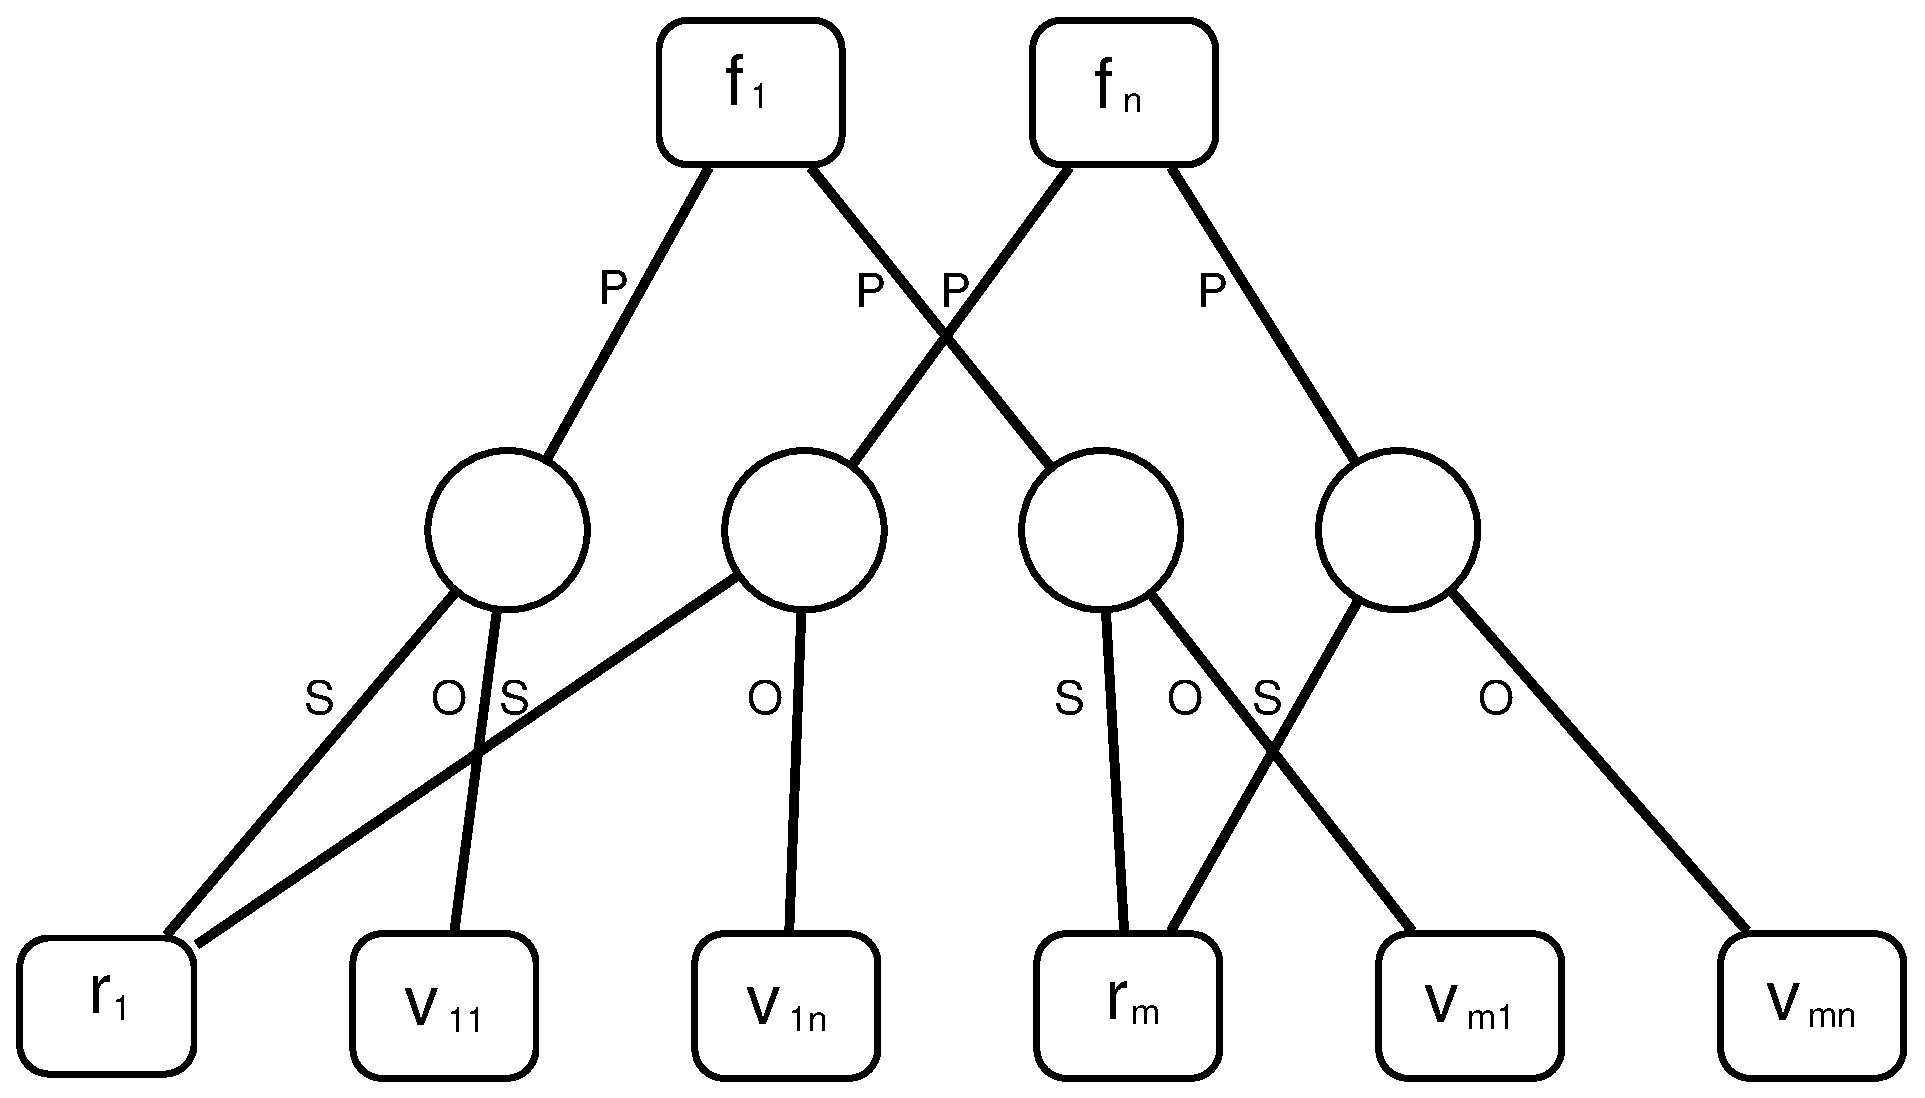
\includegraphics[width=.5\textwidth]{fig/BG-relational-nominal.eps}
\end{center}
\caption{\label{fig:BG-relational-nominal} }
\end{figure}

For relational tables with binary (boolean) features, the RDF representation can be more compact. In some applications, only cells with positive (``1") values are of interest. In this case, an auxiliary predicate can be introduced to link a row and positive cell values in that row.

\begin{myexp}[\textbf{RDF bipartite graph for a binary-valued RDB with positive values}]
\label{exp:repBinRDB}
Table~\ref{tbl:binary-rel} (A) shows an $m$-by-$n$ relational table with binary features. We use an auxiliary predicate \texttt{<mentions>} to denote a positive occurrence of a feature in one row, e.g., the statement \texttt{<$r_1$> <mentions> <$f_n$>} corresponds to the value ``1" in the $n$-th feature in the first row. Consequently, the whole Table~\ref{tbl:binary-rel} (A) maps to only two RDF statements in Table~\ref{tbl:binary-rel} (B).
\end{myexp}


\begin{table}[ht]
\begin{minipage}[b]{0.38\linewidth}\begin{flushright}
\begin{tabular}{ c | c | c | c |}
\cline{2-4}
	~   & $f_1$	    & $\cdots$  & $f_n$   \\
\cline{2-4}
$r_1:$	&  0  	& $\cdots$   &    1  \\
\cline{2-4}
$\vdots$& $\vdots$  & $\ddots$  & $\vdots$\\
\cline{2-4}
$r_m:$	&  1  	& $\cdots$   &    0  \\
\cline{2-4}
\end{tabular}
\end{flushright}
\end{minipage}
\hfill
\begin{minipage}[b]{0.4\linewidth}
\begin{tabular}{c c c}
\emph{s}&   \emph{p}&  \emph{o}\\
\texttt{<$r_1$>}   &    \texttt{<mentions>}   &  \texttt{<$f_n$>}\\
\texttt{<$r_m$>}   &    \texttt{<mentions>}   &  \texttt{<$f_1$>}\\
\end{tabular}
\end{minipage}
\begin{minipage}[c]{0.4\linewidth}\centering
\vspace{0.2cm}\hspace{2.8cm}(A)
\end{minipage}
\begin{minipage}[c]{0.4\linewidth}\centering
\vspace{0.2cm}\hspace{3.5cm}(B)
\end{minipage}
\caption{\label{tbl:binary-rel} An example relational table with binary features.}
\end{table}

Using the auxiliary predicate (\texttt{<mentions>}) greatly simplifies the resulting RDF graph by reducing the number of distinct predicates from $n$, according to the process in Definition~\ref{auto-map}, to only 1. This has profound implications for developing efficient analysis and mining methods based on the RDF bipartite graph.

However, the auxiliary predicate is feasible only when linking a row node with its positive value nodes in a binary-valued scenario. If negative cell values are also of interest and needs to be included in the RDF graph, the trick shown in the following example can be performed so that we can still use a single auxiliary predicate to link both positive and negative values:

\begin{myexp}[\textbf{RDF bipartite graph for a binary-valued RDB with both positive and negative values}]
\label{binary-reverse}
Table~\ref{tbl:binary-rel-expansion} (A) is derived from Table~\ref{tbl:binary-rel} (A) by adding a reverse column for each of its original columns, i.e., for each $f_i$, $i \in [1, n]$, a reverse $f_i'$ is created where $\forall{k\in[1,m]}~,~ v_{ki} = \neg v_{ki'}$. In this way, we can use the auxiliary predicate \texttt{<mentions>} to link to negative values by using the reverse column, because, for example, \texttt{<$r_1$> <mentions> <$f_1'$>} is equivalent to asserting $\neg$(\texttt{<$r_1$> <mentions> <$f_1$>})~. Table~\ref{tbl:binary-rel-expansion} (B) shows the RDF statements based on Table~\ref{tbl:binary-rel-expansion} (A) which essentially captures information of both positive and negative values from Table~\ref{tbl:binary-rel} (A).
\end{myexp}

\begin{table}[ht]
\begin{minipage}[b]{0.4\linewidth}\begin{flushright}
\begin{tabular}{ c | c | c | c | c | c |}
\cline{2-6}
	~   & $f_1$	 &  $f_1'$  & $\cdots$  & $f_n$  &  $f_n'$ \\
\cline{2-6}
$r_1:$	&  0  &  1	& $\cdots$   &    1  & 0\\
\cline{2-6}
$\vdots$& $\vdots$ & $\vdots$  & $\ddots$  & $\vdots$ & $\vdots$\\
\cline{2-6}
$r_m:$	&  1  &  0	& $\cdots$   &    0  & 1\\
\cline{2-6}
\end{tabular}
\end{flushright}
\end{minipage}
\hfill
\begin{minipage}[b]{0.4\linewidth}
\begin{tabular}{c c c}
\emph{s}&   \emph{p}&  \emph{o}\\
\texttt{<$r_1$>}   &    \texttt{<mentions>}   &  \texttt{<$f_1'$>}\\
\texttt{<$r_1$>}   &    \texttt{<mentions>}   &  \texttt{<$f_n$>}\\
\texttt{<$r_m$>}   &    \texttt{<mentions>}   &  \texttt{<$f_1$>}\\
\texttt{<$r_m$>}   &    \texttt{<mentions>}   &  \texttt{<$f_n'$>}\\
\end{tabular}
\end{minipage}
\hspace{1.5cm}
\begin{minipage}[c]{0.4\linewidth}\centering
\vspace{0.2cm}\hspace{2.8cm}(A)
\end{minipage}
\begin{minipage}[c]{0.4\linewidth}\centering
\vspace{0.2cm}\hspace{3.5cm}(B)
\end{minipage}
\caption{\label{tbl:binary-rel-expansion} An example expanded relational table with binary features.}
\end{table}

The process of adding reverse columns to binary-valued RDB tables described in Example~\ref{binary-reverse} can be extended to nominal-valued tables as well. By doing this we can achieve the desirable property of having only one predicate in the resulting RDF graph. The process is called RDB nominal value expansion as defined below.

\begin{mydef}[\textbf{RDB nominal value expansion}]
\label{nominal-expansion}
In a nominal valued RDB table, for each feature $f_i$ taking values on the set $V_i=\{v_{i1}, v_{i2}, \ldots\}$, we define $|f_i|$ to denote the number of its distinct values, i.e. $|f_i|=|V_i|$. The RDB nominal value expansion process transforms each nominal feature $f_i$ to $|f_i|$ number of binary features ($f_{i1}, f_{i2}, \ldots, f_{i|f_i|}$). The value of $k$-th row in $f_{ij}, (j\in [1, |f_i|)$, is ``1", if and only if $f_i$ takes the value $v_{ij}$ in the $k$-th row.
\end{mydef}

\begin{myexp}[\textbf{RDB nominal value expansion}]
Table~\ref{tbl:nominal-rel-expansion} (A) shows an nominal-valued RDB table with concrete column names and values. We use the formula, Outlook=\{sunny, overcast, rainy\}, to denote the set of distinct values the feature ``Outlook" can take on. Similarly, we have Temperature=\{hot, mild, cool\}, and Humidity=\{high, low\}. Table~\ref{tbl:nominal-rel-expansion} (B) shows the resulting table after nominal value expansion based on Definition~\ref{nominal-expansion}, and based on which, we derive the RDF statements all using one single auxiliary predicate \texttt{<mentions>}, as partly shown in Table~\ref{tbl:nominal-rel-expansion} (C).
\end{myexp}

\begin{table}[ht]
\begin{minipage}[b]{0.35\linewidth}
\begin{tabular}{ c | c | c | c |}
\cline{2-4}
	~   & O	    & T  & H   \\
\cline{2-4}
$r_1:$	&    sunny & hot & high  \\
\cline{2-4}
$r_2$:  &   rainy  & cool  & low\\
\cline{2-4}
$\vdots$& \multicolumn{3}{c|}{$\vdots$}\\
\cline{2-4}
$r_m:$	&  overcast  	& mild   & low  \\
\cline{2-4}
\end{tabular}
\end{minipage}
\begin{minipage}[b]{0.55\linewidth}
\begin{tabular}{ c | c | c | c || c | c | c || c | c |}
\cline{2-9}
~     & O\_s & O\_o & O\_r & T\_h & T\_m & T\_c & H\_h & H\_l \\
\cline{2-9}
$r_1:$ & 1 & 0 & 0 & 1 & 0 & 0 & 1 & 0 \\
\cline{2-9}
$r_2:$ & 0 & 0 & 1 & 0 & 0 & 1 & 0 & 1 \\
\cline{2-9}
$\vdots$& \multicolumn{8}{c|}{$\vdots$}\\
\cline{2-9}
$r_m:$ & 0 & 1 & 0 & 0 & 1 & 0 & 0 & 1 \\
\cline{2-9}
\end{tabular}
\end{minipage}
\hspace{1.5cm}
\begin{minipage}[c]{0.35\linewidth}\centering
\vspace{0.2cm}\hspace{1.5cm}(A)
\end{minipage}
\begin{minipage}[c]{0.55\linewidth}\centering
\vspace{0.2cm}\hspace{1.5cm}(B)
\end{minipage}
\begin{minipage}[b]{\linewidth}\centering
\begin{tabular}{c c c}
&&\\
\emph{s}&   \emph{p}&  \emph{o}\\
\texttt{<$r_1$>}   &    \texttt{<mentions>}   &  \texttt{<O\_s>}\\
\texttt{<$r_1$>}   &    \texttt{<mentions>}   &  \texttt{<T\_h>}\\
\texttt{<$r_1$>}   &    \texttt{<mentions>}   &  \texttt{<H\_h>}\\
\texttt{<$r_2$>}   &    \texttt{<mentions>}   &  \texttt{<O\_r>}\\
\multicolumn{3}{c}{$\cdots$}\\
\multicolumn{3}{c}{(C)}\\
\end{tabular}
\end{minipage}
\caption{\label{tbl:nominal-rel-expansion} An example nominal-valued relational table after nominal value expansion. (A) shows the original table where O stands for ``outlook", T for ``temperature" and "H" for humidity. (B) shows the expanded table. (C) shows the corresponding RDF triples derived from (B).}
\end{table}

\section{Combining Data Graphs and Ontology Graphs}

In order to seamlessly interface data and domain knowledge in a mining framework, the information in both sources needs to be first associated. This is achieved by the process called \emph{semantic annotation}. Semantic Annotation aims at assigning to the basic element of data links to formal semantic descriptions. Such elements should constitute the semantics of their source, for example, named entities in a document, certain part of an image depicting someone's head portrait.

Semantic annotation is crucial in realizing semantic data mining by bridging formal semantics in domain knowledge with data. What is more important, semantic annotation also enables a spectrum of new applications, such as indexing, retrieval, inference, categorization, query answering etc. These applications can also play vital roles in semantic data mining.

In the following, we assume data is annotated, meaning the links between entities in the data and formal semantic descriptions (such as those in ontologies) are established. A unified graph incorporating information from both data and domain knowledge can be created. Data mining algorithms dealing with such graph enjoys the benefits of a seamless integration of domain semantics. The following example shows the combination of an ontology graph and a data graph.

%\textbf{b) Domain Semantics--driven Mapping Generation}: The second approach generates mappings from RDB to RDF by incorporating domain semantics that is often implicit or not captured at all in the RDB schema. The explicit modeling of domain semantics, often modeled as a domain ontology. The domain ontology may be pre--existing and sourced from public resources.

\begin{myexp}[\textbf{Combining an ontology graph and a data graph}]
Figure~\ref{fig:onto-and-data} (A) shows an simple ontology in some domain with only subsumption relationship defined for five entities (A--B). Figure~\ref{fig:onto-and-data} (B) shows a binary-valued RDB table in the same domain with the set of entities serving as features. We use the same entity labels in the ontology and the RDB table because we assume the mapping between ontology nodes and table features are pre-assigned or established by automatic annotation. Figure~\ref{fig:hypergraph-combined} (B) shows the RDF statements derived from both the ontology and the RDB table. Figure~\ref{fig:hypergraph-combined} (A) demonstrates the combined RDF bipartite graph.

Positions of nodes in Figure~\ref{fig:hypergraph-combined} (A) can be rearranged to form Figure~\ref{fig:bipartitegraph-weighted}. This graph demonstrates a tripartite structure where row nodes ($r_1$--$r_5$) fall on one partition, column nodes (A--E) another, and statement nodes in between. A plethora of graph-theoretic algorithms and graph mining techniques can be leveraged to analyze the configuration of connecting paths in this graph to answer questions such as grouping in rows and columns (for solving the the task of clustering and association mining respectively). Predicate nodes can serve as a sign to introduce different weights to paths in order to distinguish different semantic information conveyed by those predicates.

Edges and statement nodes in Figure~\ref{fig:bipartitegraph-weighted} are depicted in two colors to signify their sources of origin. Red edges and nodes denote information from the data (RDB table), and blue ones from the ontology. It can be seen from the graph that the contribution of ontology is to introduce extra paths with different semantic types (The data is structured under the ``mentions" relationship and the ontology is structured under the subsumption relationship). A mining algorithm that is able to deal with the data graph can be naturally extended without major modification to handle domain knowledge coded in the ontology.
\end{myexp}

\begin{figure}[tbh]
\begin{minipage}[c]{.45\textwidth}\centering
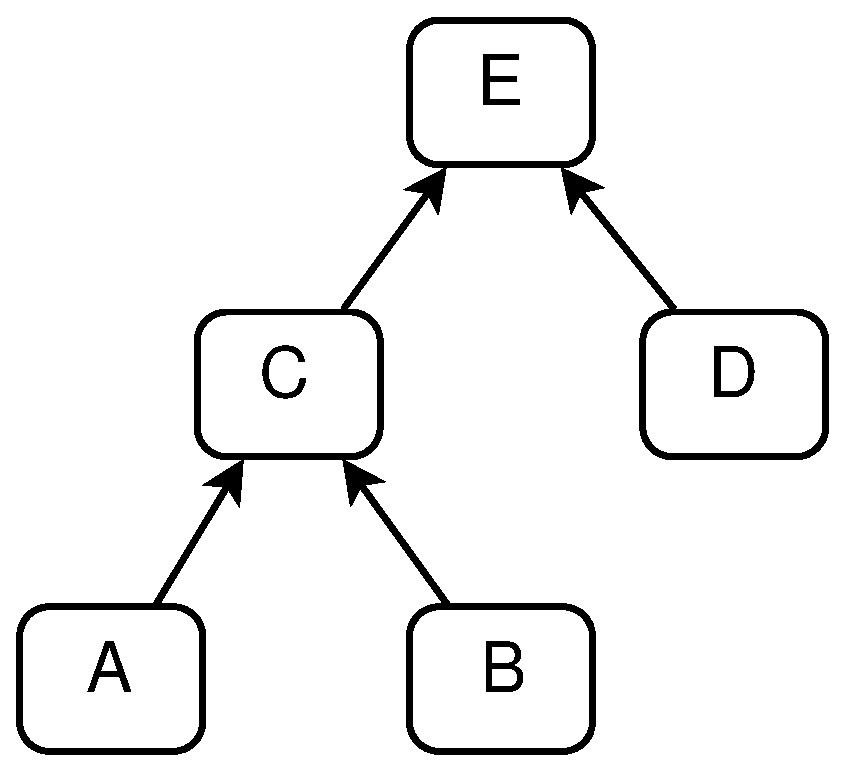
\includegraphics[width=.5\linewidth]{fig/simple-onto.eps}
\end{minipage}
\begin{minipage}[b]{.45\textwidth}\centering
    \begin{tabular}{ c | c | c | c | c | c |}
    \cline{2-6}
    	~ & A & B & C & D & E\\
    \cline{2-6}
    $r_1:$& 1 & 1 & 0 & 0 & 0 \\
    \cline{2-6}
    $r_2:$& 1 & 1 & 1 & 0 & 0 \\
    \cline{2-6}
    $r_3:$& 0 & 1 & 1 & 0 & 0 \\
    \cline{2-6}
    $r_3:$& 0 & 0 & 0 & 1 & 0 \\
    \cline{2-6}
    \end{tabular}
\end{minipage}
\begin{minipage}[c]{0.4\linewidth}\centering
\vspace{0.2cm}\hspace{2cm}(A)
\end{minipage}
\begin{minipage}[c]{0.4\linewidth}\centering
\vspace{0.2cm}\hspace{4cm}(B)
\end{minipage}
\caption{\label{fig:onto-and-data} An example of a binary-valued relational table (B) about five concepts (``A"--``E"), and the ontological relationship among these concepts shown as a directed graph (A).}
\end{figure}

\begin{figure}[tbh]
\begin{center}
\begin{tabular}{c  c}
\multirow{12}{*}{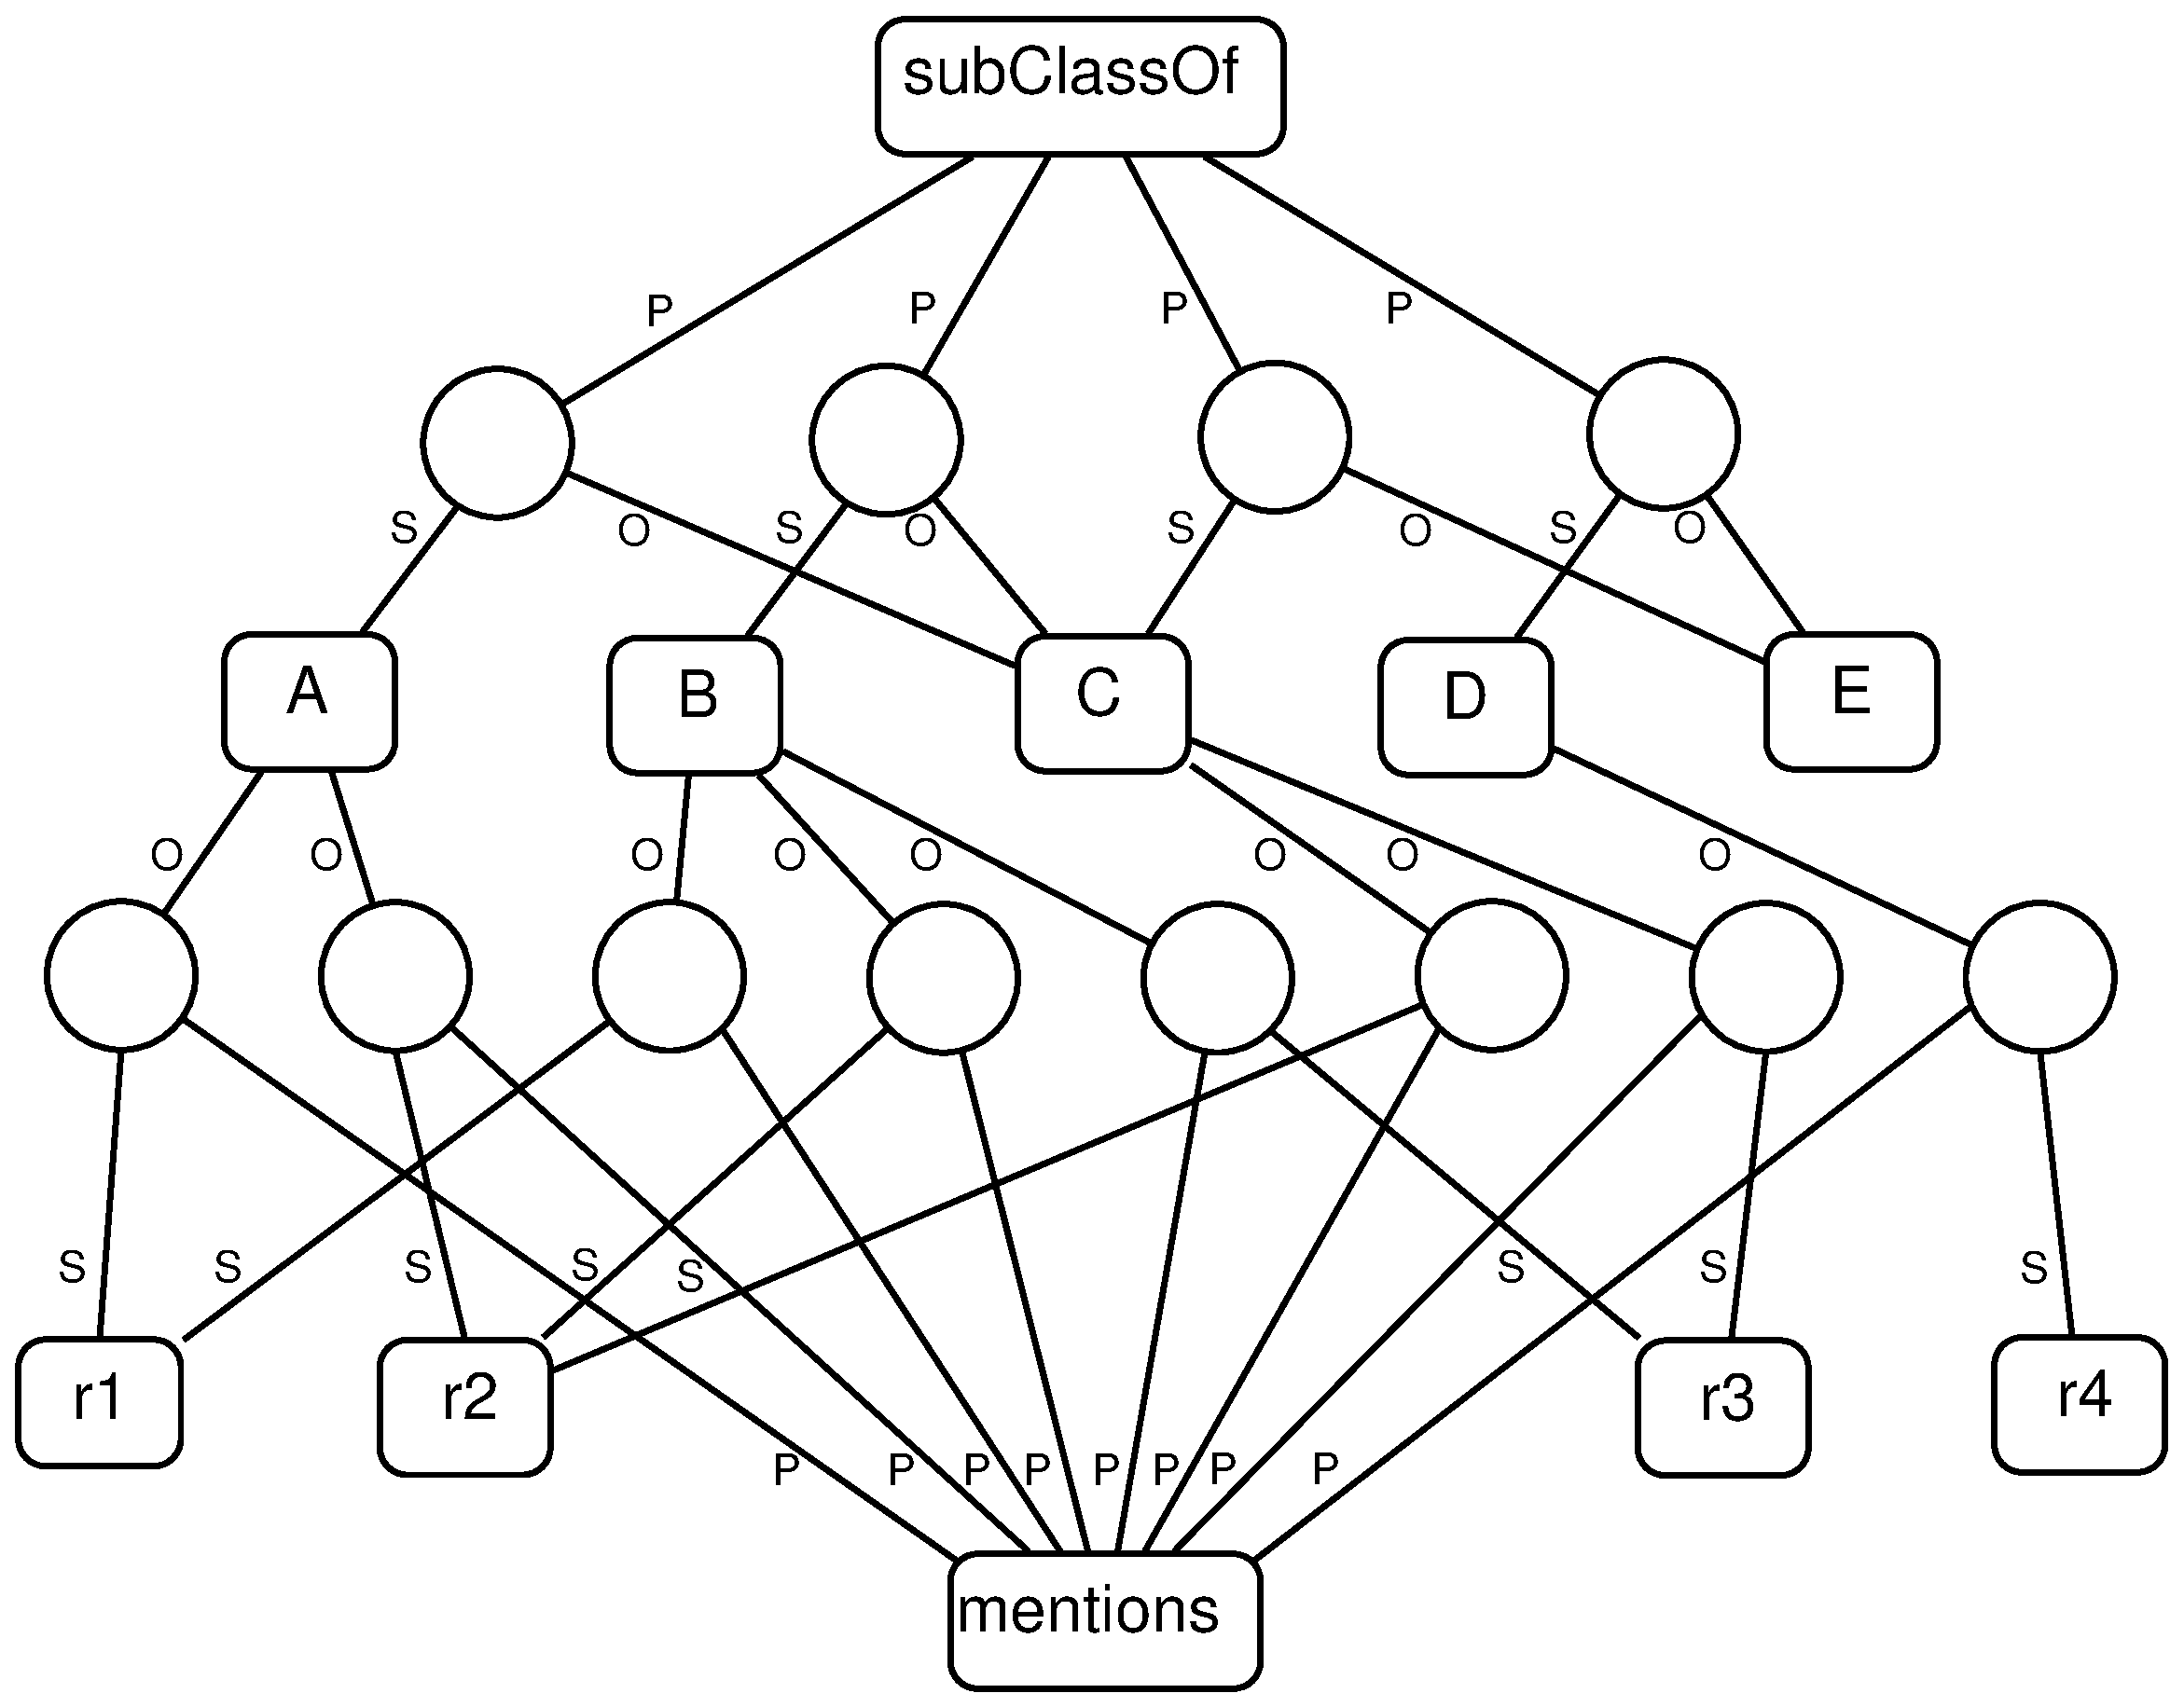
\includegraphics[width=.55\textwidth]{fig/hypergraph_mining.eps}} & \emph{~~~s \hfill p\hfill o~~~}\\
& \texttt{<A>~~<subClassOf>~~<C>}\\
& \texttt{<B>~~<subClassOf>~~<C>}\\
& \texttt{<C>~~<subClassOf>~~<E>}\\
& \texttt{<D>~~<subClassOf>~~<E>}\\
& \\
& \texttt{<r1>\;~~<mentions>\;~~<A>}\\
& \texttt{<r1>\;~~<mentions>\;~~<B>}\\
& \texttt{<r2>\;~~<mentions>\;~~<A>}\\
& \texttt{<r2>\;~~<mentions>\;~~<B>}\\
& \texttt{<r2>\;~~<mentions>\;~~<C>}\\
& \texttt{<r3>\;~~<mentions>\;~~<B>}\\
& \texttt{<r3>\;~~<mentions>\;~~<C>}\\
& \texttt{<r4>\;~~<mentions>\;~~<D>}\\
& \\
& \\
(A) & (B)\\
\end{tabular}
\end{center}
\caption{\label{fig:hypergraph-combined} The RDF bipartite graph representation (A) given triples shown in (B) based on the information described in Figure~\ref{fig:onto-and-data}.}
\end{figure}

\begin{figure}[tbh]
\begin{center}
\includegraphics[width=.6\textwidth]{fig/hypergraph_mining-bipartite-weighted.eps}
\end{center}
\caption{\label{fig:bipartitegraph-weighted} This figure show that, grouping the nodes according to whether they are row elements or column elements in Figure~\ref{fig:onto-and-data} (B), the bipartite graph shown in Figure~\ref{fig:hypergraph-combined} (A) can be further transformed to a tripartite graph.}
\end{figure}

\subsection{Representing Different Kinds of Ontological Semantics}
\label{sec:rosg}

%In our preliminary work, we have showed a way to represent ontology annotated data in hypergraphs which help discovering semantic associations.  If the domain knowledge is defined as formal ontologies, it is a natural thinking to use graphs to represent the domain knowledge as well. To formally represent domain knowledge using graphs, it is important to different types of formal semantics in a systematic way.

In order to leverage the increasingly larger and richer collection of domain ontologies, especially in scientific fields such as the biomedical domain, we propose to develop methods for the representation of different types of ontological semantics which supports efficient semantic data mining. We propose to develop a weighting scheme to distinguish paths in the RDF bipartite graph that contains these different relationships such as class subsumption, part\_of, and other general or domain--specific properties. %(e.g., Drug \textit{treat} Disease).

\begin{myexp}[\textbf{Assigning weights to different relationship}]
Figure~\ref{fig:hypergraph_mining-comp} shows an example of RDF bipartite graph representing information on peoples (A--E) where multiple relationships can be identified to link them. E.g., A, B, C and D are linked by the coauthorship relationship, while D and E are linked by the more general collaboration relationship (in fact, coauthorship is defined as a sub-property of collaboration in the ontology). A, B and C are professors, D and E are PhD students, and both professors and PhD students are researchers. In this complex lattice of relationships, we hope to distinguish these relationships by assigning task--specific weights to the related paths (e.g., as conveyed by different colorings in the graph). In order to achieve this, we propose to develop a framework for guiding the (semi-) automatic assignment of weights.
\end{myexp}

\begin{figure}[tbh]
\begin{center}
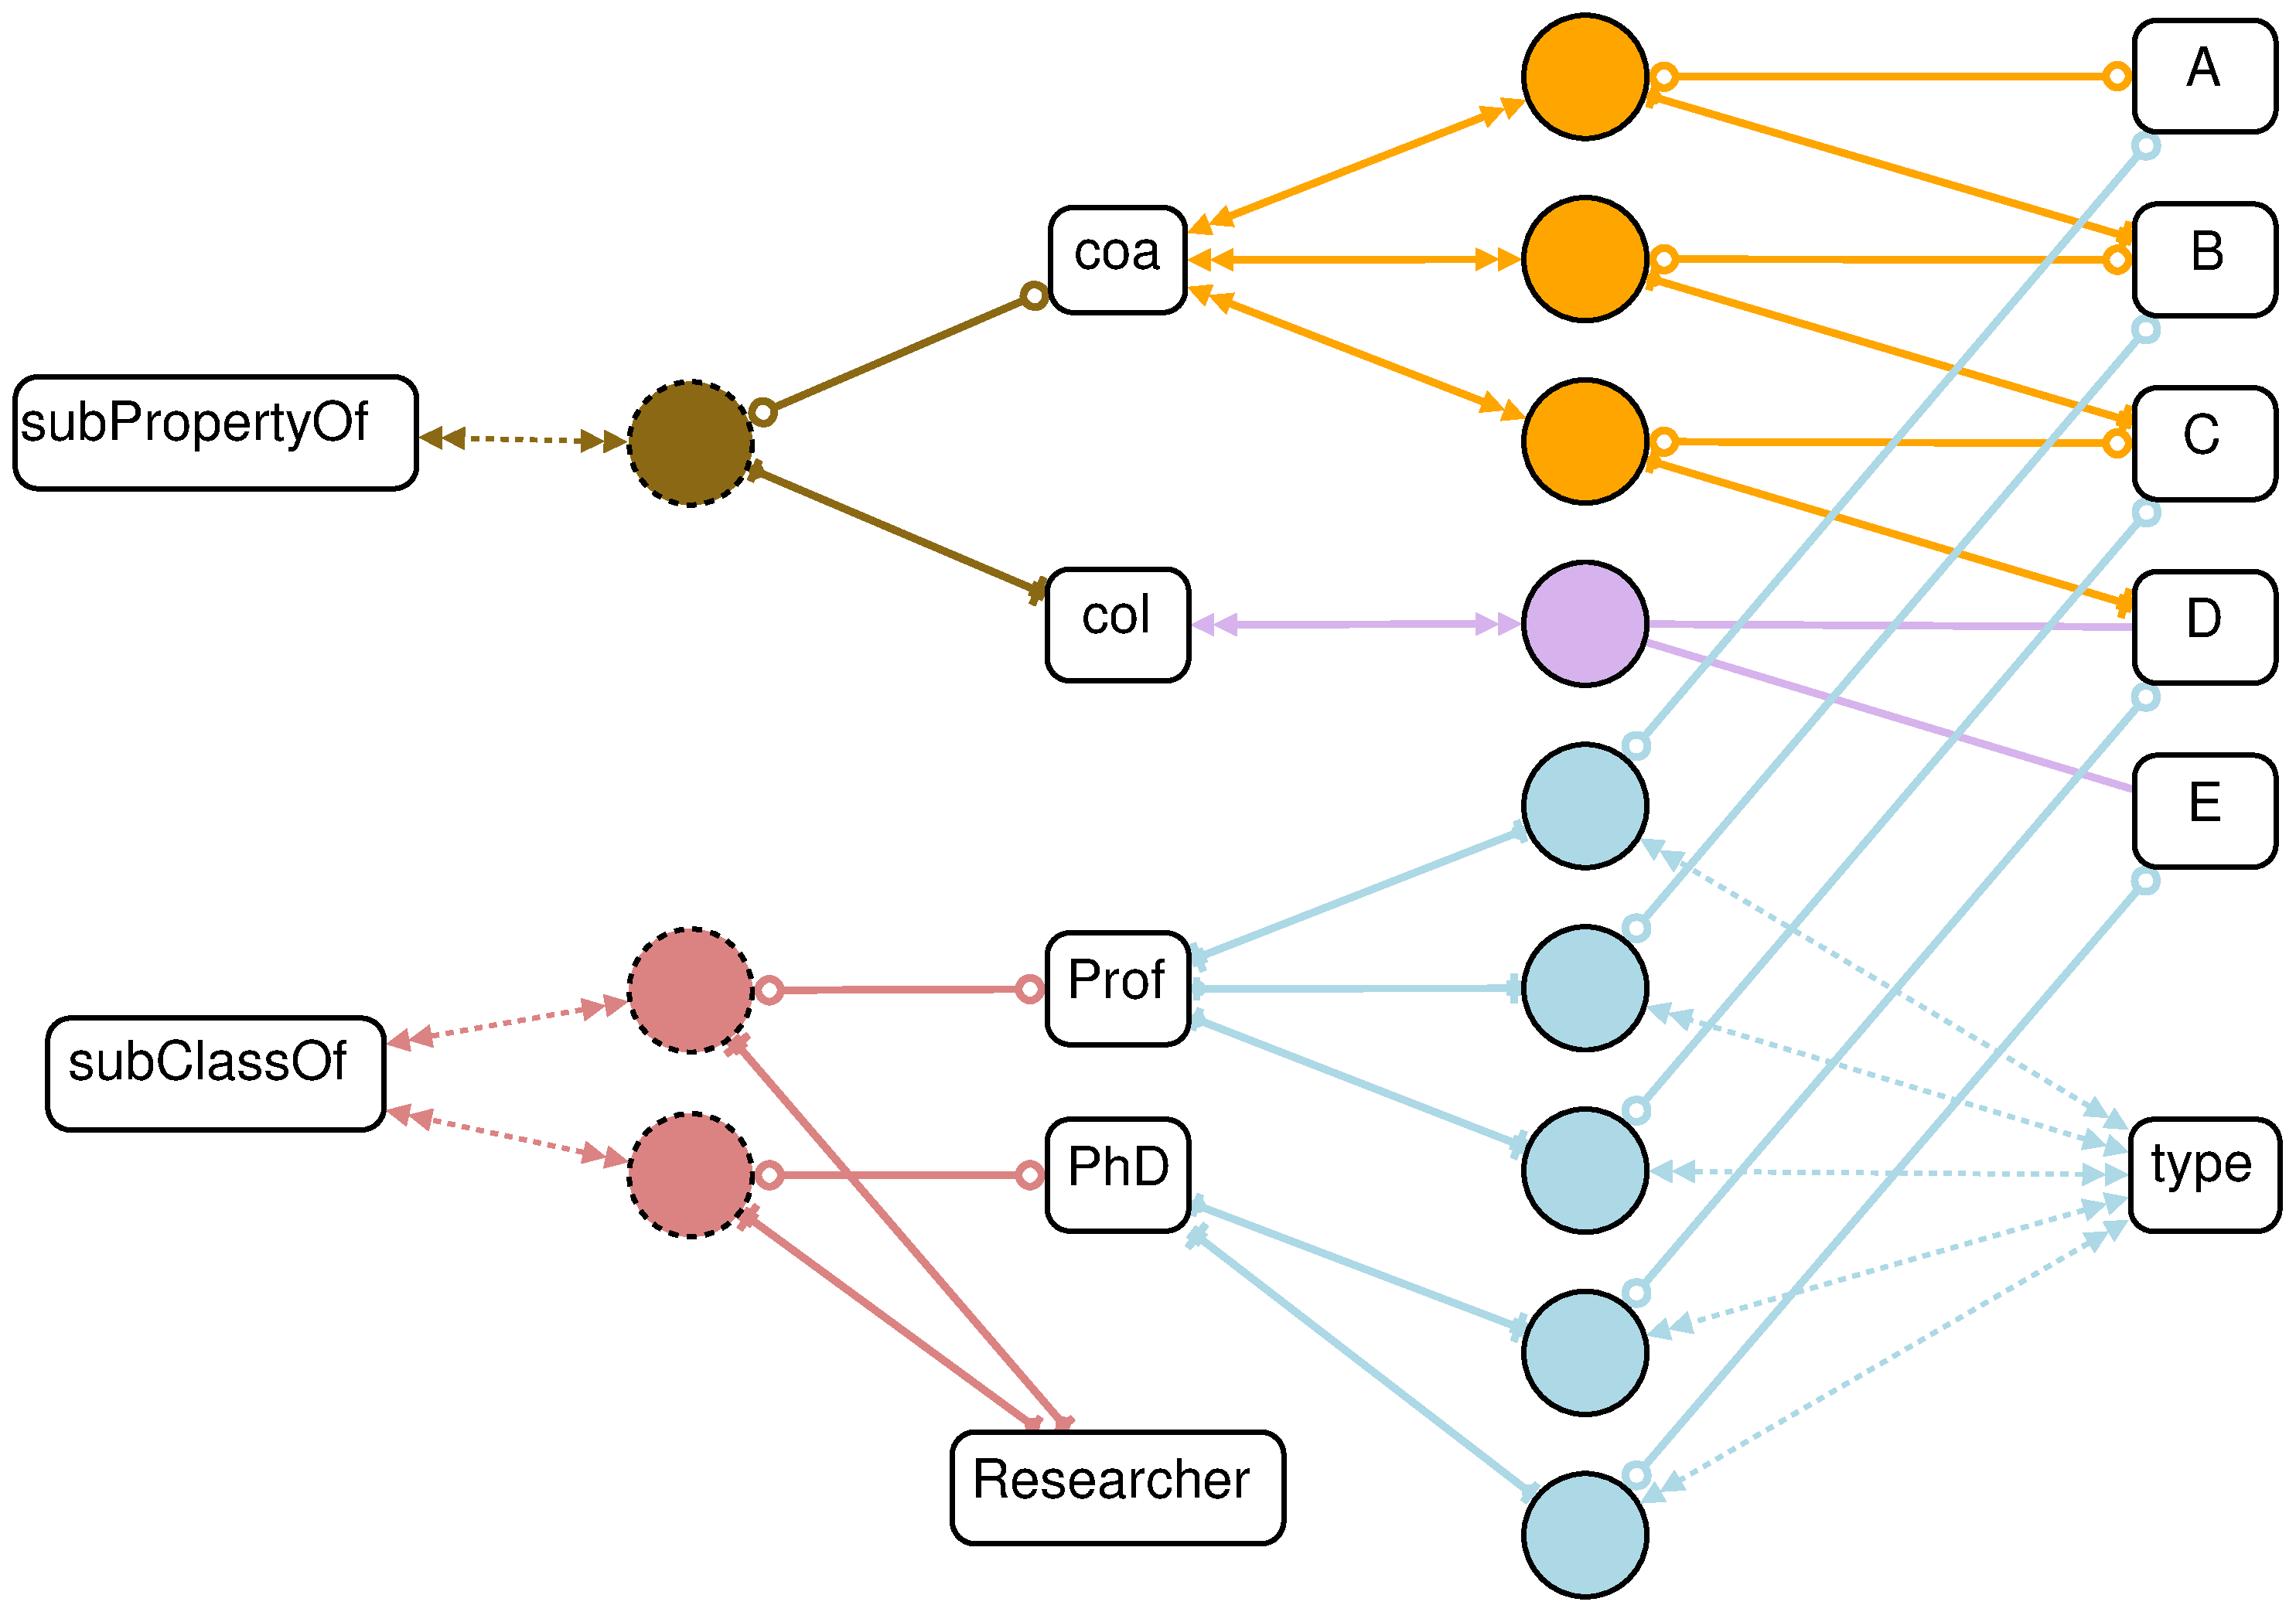
\includegraphics[width=.65\textwidth]{fig/hypergraph_mining-comp.eps}
\end{center}
\caption{\label{fig:hypergraph_mining-comp} }
\end{figure}
